%=========================================================
% Capítulo 8 — A assimilação variacional (3DVar e 4DVar)
%=========================================================
\chapter{A assimilação variacional (3DVar e 4DVar)}
\label{ch:variacional}

\noindent\textbf{Resumo:}
Neste capítulo, apresentamos a formulação variacional da assimilação de dados, onde a análise é obtida como o mínimo de uma função custo.  
O método 3DVar resolve o problema em um instante de tempo, enquanto o 4DVar estende o ajuste para um intervalo temporal, utilizando a dinâmica do modelo.  
Essas abordagens constituem a base de muitos sistemas operacionais de previsão numérica do tempo.

%---------------------------------------------------------
\section{Motivação}
A assimilação variacional nasce do mesmo princípio do filtro de Kalman: combinar coerentemente background e observações, ponderados por seus erros.  
Mas, em vez de uma atualização recursiva, o método variacional formula o problema como uma \emph{minimização global} da função custo:
\begin{equation}
J(\mathbf{x}) = (\mathbf{x} - \mathbf{x}_b)^\top \mathbf{B}^{-1} (\mathbf{x} - \mathbf{x}_b)
+ (\mathbf{y} - \mathbf{H}\mathbf{x})^\top \mathbf{R}^{-1} (\mathbf{y} - \mathbf{H}\mathbf{x}).
\label{eq:J-3DVar}
\end{equation}
Essa forma é idêntica à função custo da análise estatística apresentada no Capítulo~\ref{ch:formulacao-estatistica}.  
A diferença é que, agora, resolvemos a minimização de forma iterativa e, no caso 4D, incorporamos a evolução temporal do modelo.

%---------------------------------------------------------
\section{O método 3DVar}
O \textbf{3DVar} (\emph{Three-Dimensional Variational Assimilation}) considera todas as observações em um instante fixo de tempo.  
O gradiente da função custo é:
\begin{equation}
\nabla J = \mathbf{B}^{-1} (\mathbf{x} - \mathbf{x}_b)
- \mathbf{H}^\top \mathbf{R}^{-1} (\mathbf{y} - \mathbf{H}\mathbf{x}).
\label{eq:grad3dvar}
\end{equation}
O mínimo é obtido quando $\nabla J = 0$, o que leva exatamente à solução de análise dada pela equação de Kalman estática:
\[
\mathbf{x}_a = \mathbf{x}_b + \mathbf{K} (\mathbf{y} - \mathbf{H}\mathbf{x}_b),
\]
com $\mathbf{K}$ definido como em \eqref{eq:kalman-gain}.  
A diferença é que, em 3DVar, não se calcula explicitamente $\mathbf{K}$; em vez disso, resolve-se \eqref{eq:J-3DVar} iterativamente, com métodos como \textbf{Conjugate Gradient} ou \textbf{L-BFGS}.

\begin{figure}[h!]
\centering
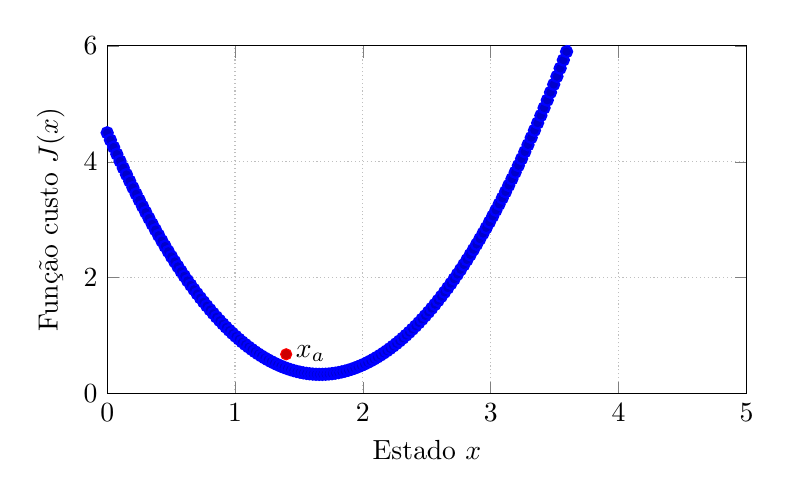
\begin{tikzpicture}
\begin{axis}[
  width=0.8\linewidth, height=6cm,
  xlabel={Estado $x$}, ylabel={Função custo $J(x)$},
  xmin=0, xmax=5, ymin=0, ymax=6,
  grid=both, grid style={densely dotted},
  legend style={at={(0.98,0.98)},anchor=north east,draw=none}
]
  \addplot+[domain=0:5, samples=200, thick] {(x-1)^2/2 + (2-x)^2};
  \addplot+[only marks,mark=*] coordinates {(1.4,0.68)}; 
  \node[anchor=west] at (axis cs:1.4,0.7) {$x_a$};
\end{axis}
\end{tikzpicture}
\caption{Interpretação geométrica da análise 3DVar: o ponto mínimo de $J(x)$ representa o estado mais provável, conciliando modelo e observações.}
\label{fig:3dvar-cost}
\end{figure}

%---------------------------------------------------------
\section{O método 4DVar}
O \textbf{4DVar} (\emph{Four-Dimensional Variational Assimilation}) estende o conceito para um período de tempo $[t_0, t_n]$.  
A função custo incorpora todas as observações disponíveis ao longo desse intervalo, aplicando a dinâmica do modelo como restrição:
\begin{equation}
J(\mathbf{x}_0) = (\mathbf{x}_0 - \mathbf{x}_b)^\top \mathbf{B}^{-1} (\mathbf{x}_0 - \mathbf{x}_b)
+ \sum_{k=0}^{n} (\mathbf{y}_k - \mathbf{H}_k \mathbf{M}_{k,0} \mathbf{x}_0)^\top
\mathbf{R}_k^{-1} (\mathbf{y}_k - \mathbf{H}_k \mathbf{M}_{k,0} \mathbf{x}_0),
\label{eq:J-4DVar}
\end{equation}
onde $\mathbf{M}_{k,0}$ é o modelo linearizado que propaga o estado inicial $\mathbf{x}_0$ até o tempo $t_k$.

Assim, o 4DVar procura o estado inicial que, ao ser evoluído pelo modelo, melhor ajusta todas as observações no período.

%---------------------------------------------------------
\section{O papel do operador adjunto}
A minimização de \eqref{eq:J-4DVar} requer o cálculo eficiente do gradiente $\nabla J$.  
Como o modelo é geralmente de alta dimensão, calcular derivadas diretas é inviável.  
Utiliza-se então o \textbf{operador adjunto} $\mathbf{M}^\top$, que propaga as sensibilidades de volta no tempo:
\[
\nabla J = \mathbf{B}^{-1} (\mathbf{x}_0 - \mathbf{x}_b)
- \sum_{k=0}^{n} \mathbf{M}_{k,0}^\top \mathbf{H}_k^\top \mathbf{R}_k^{-1}
(\mathbf{y}_k - \mathbf{H}_k \mathbf{M}_{k,0} \mathbf{x}_0).
\]
Esse cálculo adjunto permite a otimização iterativa mesmo em sistemas com milhões de variáveis, como os modelos atmosféricos globais.

\begin{figure}[h!]
\centering
\begin{tikzpicture}
\begin{axis}[
  width=0.9\linewidth, height=6cm,
  xlabel={tempo}, ylabel={diferença modelo–observação},
  xmin=0, xmax=10, ymin=-3, ymax=3,
  grid=both, grid style={densely dotted}
]
  \addplot+[domain=0:10, samples=200, thick] {2*sin(deg(0.7*x)) - 0.5*x};
  \addplot+[domain=0:10, samples=200, thick, dashed, color=brandA] {2*sin(deg(0.7*x))};
  \legend{modelo, observações}
\end{axis}
\end{tikzpicture}
\caption{O 4DVar ajusta o estado inicial para que a trajetória do modelo se alinhe com as observações ao longo de todo o intervalo.}
\label{fig:4dvar}
\end{figure}

%---------------------------------------------------------
\section{Comparação entre 3DVar, 4DVar e EnKF}
\begin{center}
\begin{tabular}{lccc}
\toprule
\textbf{Característica} & \textbf{3DVar} & \textbf{4DVar} & \textbf{EnKF} \\
\midrule
Dependência temporal & Instantânea & Intervalo $[t_0,t_n]$ & Sequencial \\
Linearização do modelo & Não & Necessária & Não \\
Representação de erro & Estatística fixa ($B$) & Linearizada via modelo & Amostrada (ensemble) \\
Custo computacional & Moderado & Elevado & Escalável \\
Uso do adjunto & Não & Sim & Não \\
\bottomrule
\end{tabular}
\end{center}

Cada método tem suas vantagens:
\begin{itemize}
  \item o \textbf{3DVar} é simples e eficiente, adequado para ciclos rápidos;
  \item o \textbf{4DVar} fornece a melhor coerência temporal, ao custo de maior complexidade;
  \item o \textbf{EnKF} é flexível e ideal para modelos complexos e não lineares.
\end{itemize}

%---------------------------------------------------------
\section{Síntese}
O método variacional reformula a assimilação como um problema de otimização no espaço do modelo.  
Enquanto o Filtro de Kalman atualiza explicitamente o estado, o 4DVar busca o estado inicial ótimo cujo desenvolvimento temporal é mais consistente com as observações.  
A equivalência entre o filtro e o método variacional foi demonstrada por Lorenc (1986), unificando os dois paradigmas sob a mesma base estatística.

No próximo capítulo, exploraremos os \emph{métodos híbridos}, que combinam as vantagens do 4DVar e do EnKF para obter análises consistentes, dinâmicas e estatisticamente robustas.

% Fim do Capítulo 8
